\chapter{Results}

\section{Experiment 1}
The mean sentence score for each talker across all listeners is given in Figure~\ref{fig:ExpOneBarplot}.  As predicted, 


\begin{figure}[htbp]
	\begin{centering}
	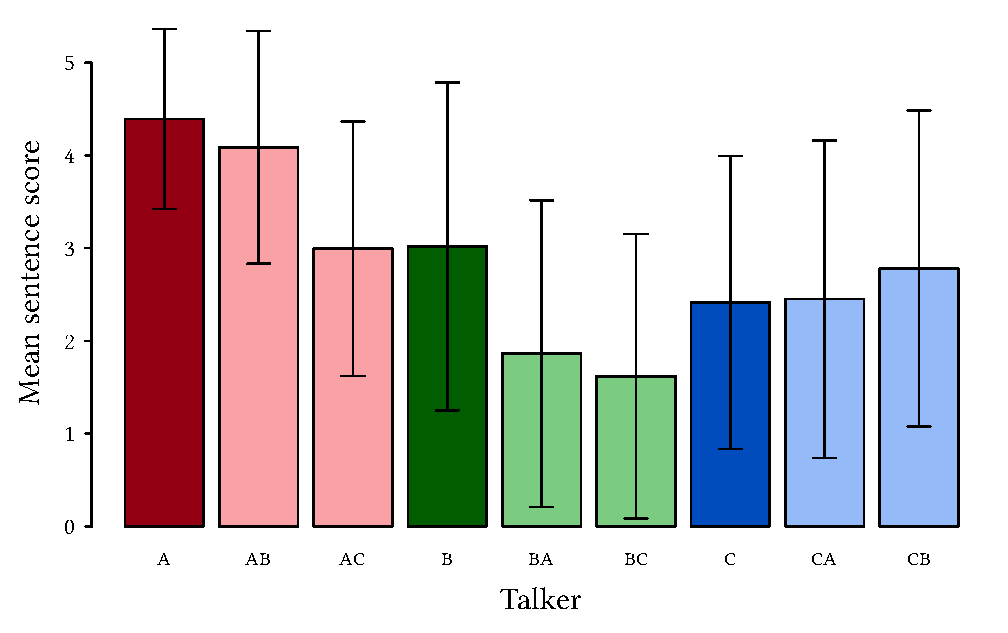
\includegraphics{figures/results/ExpOneBarplot.eps}
	\caption[Barplot of mean sentence scores for Experiment~1]{Barplot of mean sentence scores for Experiment~1.  Error bars are ±1 standard error.  See Section~\ref{sec:xxx} for explanation of talker codes.\label{fig:ExpOneBarplot}}
	\end{centering}
\end{figure}


\begin{table}
	\caption[Experiment~1 statistical model]{Summary of fixed effect predictors for the statistical model of Experiment~1.\label{tab:ExpOneFixedEff}}
	\centering
	\begin{tabu}{Xrrrl}
		\toprule
		\rowfont{\bfseries}\multicolumn{5}{l}{Summary of fixed effects (N=1440; log-likelihood=-2554)}\\\\
		\rowfont{\bfseries}Predictor & Coefficient & \textit{SE} & Wald \textit{Z} & \textit{p}\\
		\midrule
		Intercept             &  4.382 & (0.132) &  33.19 &<10⁻¹⁶\\
		resynth=TRUE          & −0.666 & (0.077) &  −8.64 &<10⁻¹⁶\\
		segmentalDonor=\ac{b} & −1.679 & (0.089) & −18.82 &<10⁻¹⁶\\
		segmentalDonor=\ac{c} & −1.274 & (0.090) & −14.18 &<10⁻¹⁶\\
		prosodicDonor=\ac{b}  &  0.315 & (0.089) &   3.54 &<10⁻³\\
		prosodicDonor=\ac{c}  & −0.635 & (0.088) &  −7.19 &<10⁻¹¹\\
		\bottomrule
	\end{tabu}
\end{table}


\section{Experiment 2}

Experiment~2 results.
